\chapter{Persistence}

    \section{I/O devices}

    \sssc{Prototypical System Architecture}

    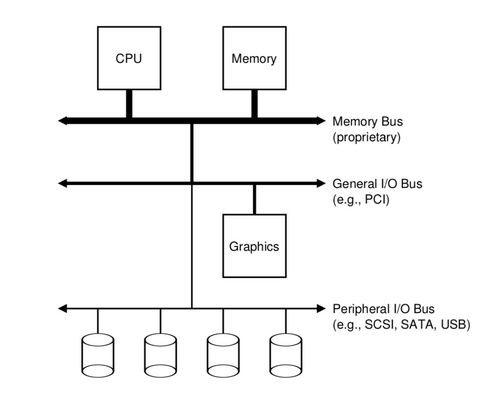
\includegraphics[width=0.6\textwidth]{chapters/Persistence/persistence/psa.png}

    CPU and Memory are connected to the \textbf{Memory Bus}. Other devices like graphic card 
    are connected to the system via a general \textbf{I/O bus}, which should 
    be PCI(or its derivatives). There is even lower bus called \textbf{peripheral bus}, such that 
    \textbf{SCSI,SATA} or \textbf{USB} can be attached here. Those connect slow devices to the 
    system, including disks, mice and keyboards.

    The idea is that: components that demand high performance are nearer the CPU. Lower 
    performance components are further away.


    \sssc{Modern System Architecture}

    Modern systems use specialized chipsets and faster point-to-point interconnects to 
    improve performance.

    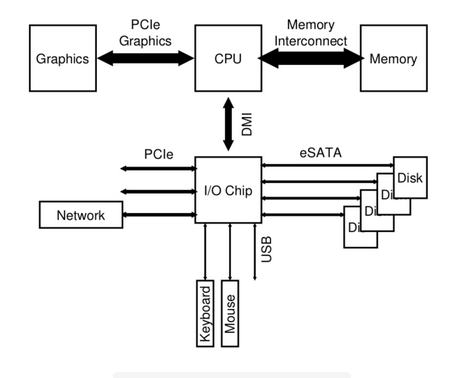
\includegraphics[width=0.6\textwidth]{chapters/Persistence/persistence/msa.png}

    

